\documentclass[journal,12pt,twocolumn]{IEEEtran}

\usepackage{enumitem}
\usepackage{amsmath}
\usepackage{amssymb}
\usepackage{gensymb}
\usepackage{graphicx}
\usepackage{txfonts}         
\usepackage{listings}
\usepackage{lstautogobble}
\usepackage{mathtools}
\usepackage{bm}
\usepackage{hyperref}
\usepackage{polynom}
\usepackage{siunitx}
\usepackage{verbatim}
\usepackage[siunitx]{circuitikz}

\newcommand{\solution}{\noindent \textbf{Solution: }}
\providecommand{\pr}[1]{\ensuremath{\Pr\left(#1\right)}}
\providecommand{\brak}[1]{\ensuremath{\left(#1\right)}}
\providecommand{\cbrak}[1]{\ensuremath{\left\{#1\right\}}}
\providecommand{\sbrak}[1]{\ensuremath{\left[#1\right]}}
\providecommand{\mean}[1]{E\left[ #1 \right]}
\providecommand{\var}[1]{\mathrm{Var}\left[ #1 \right]}
\providecommand{\der}[1]{\mathrm{d} #1}
\providecommand{\gauss}[2]{\mathcal{N}\ensuremath{\left(#1,#2\right)}}
\providecommand{\mbf}{\mathbf}
\providecommand{\abs}[1]{\left\vert#1\right\vert}
\providecommand{\norm}[1]{\left\lVert#1\right\rVert}
\providecommand{\z}[1]{{\mathcal{Z}}\cbrak{#1}}
\providecommand{\ztrans}{\overset{\mathcal{Z}}{ \rightleftharpoons}}
\providecommand{\system}[1]{\overset{\mathcal{#1}}{ \longleftrightarrow}}
\providecommand{\parder}[2]{\frac{\partial}{\partial #2} \brak{#1}}
\providecommand{\rect}[1]{\mathrm{rect}\ensuremath{\left(#1\right)}}
\providecommand{\sinc}[1]{\mathrm{sinc}\ensuremath{\left(#1\right)}}

\let\StandardTheFigure\thefigure
\let\vec\mathbf

\numberwithin{equation}{section}
\numberwithin{figure}{section}
\renewcommand{\thefigure}{\theenumi}
\renewcommand\thesection{\arabic{section}}

\newcommand{\myvec}[1]{\ensuremath{\begin{pmatrix}#1\end{pmatrix}}}
\newcommand{\mymat}[1]{\ensuremath{\begin{bmatrix}#1\end{bmatrix}}}
\newcommand{\mydet}[1]{\ensuremath{\begin{vmatrix}#1\end{vmatrix}}}
\newcommand{\define}{\stackrel{\triangle}{=}}

\DeclareMathOperator*{\argmin}{arg\,min}
\DeclareMathOperator*{\argmax}{arg\,max}

\makeatletter
\def\pld@CF@loop#1+{%
    \ifx\relax#1\else
        \begingroup
          \pld@AccuSetX11%
          \def\pld@frac{{}{}}\let\pld@symbols\@empty\let\pld@vars\@empty
          \pld@false
          #1%
          \let\pld@temp\@empty
          \pld@AccuIfOne{}{\pld@AccuGet\pld@temp
                            \edef\pld@temp{\noexpand\pld@R\pld@temp}}%
           \pld@if \pld@Extend\pld@temp{\expandafter\pld@F\pld@frac}\fi
           \expandafter\pld@CF@loop@\pld@symbols\relax\@empty
           \expandafter\pld@CF@loop@\pld@vars\relax\@empty
           \ifx\@empty\pld@temp
               \def\pld@temp{\pld@R11}%
           \fi
          \global\let\@gtempa\pld@temp
        \endgroup
        \ifx\@empty\@gtempa\else
            \pld@ExtendPoly\pld@tempoly\@gtempa
        \fi
        \expandafter\pld@CF@loop
    \fi}
\def\pld@CMAddToTempoly{%
    \pld@AccuGet\pld@temp\edef\pld@temp{\noexpand\pld@R\pld@temp}%
    \pld@CondenseMonomials\pld@false\pld@symbols
    \ifx\pld@symbols\@empty \else
        \pld@ExtendPoly\pld@temp\pld@symbols
    \fi
    \ifx\pld@temp\@empty \else
        \pld@if
            \expandafter\pld@IfSum\expandafter{\pld@temp}%
                {\expandafter\def\expandafter\pld@temp\expandafter
                    {\expandafter\pld@F\expandafter{\pld@temp}{}}}%
                {}%
        \fi
        \pld@ExtendPoly\pld@tempoly\pld@temp
        \pld@Extend\pld@tempoly{\pld@monom}%
    \fi}
\makeatother

\lstset {
	frame=single, 
	breaklines=true,
	columns=fullflexible,
	autogobble=true
}             
                               
\title{Fourier Series \\ \Large EE3900: Linear Systems and Signal Processing \\ \large Indian Institute of Technology Hyderabad}
\author{Aayush Prabhu \\ \normalsize AI21BTECH11002}

\begin{document}

	\maketitle

	\section{Periodic Function}
	Let 
	\begin{align}
		x(t) &= A_0\abs{\sin\brak{2\pi f_0 t}}
		\label{eq:10-orig-diff-def}
	\end{align}

	\begin{enumerate}[label=\thesection.\arabic*,ref=\thesection.\theenumi]
	\item Plot $x(t)$
	
	\solution Download the following Python code that plots Fig. \ref{fig-1.1}.
	\begin{lstlisting}
		wget https://github.com/Ankit-Saha-2003/EE3900/raw/main/Fourier/codes/1.1.py
	\end{lstlisting}
	
	Run the code by executing
	\begin{lstlisting}
		python 1.1.py
	\end{lstlisting}

	\begin{figure}[!ht]
		\centering
		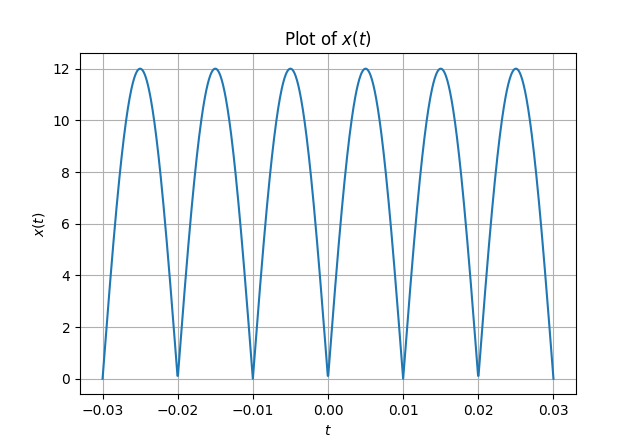
\includegraphics[width=\columnwidth]{./figs/1.1.png}
		\caption{Plot of $x(t)$}
		\label{fig-1.1}	
	\end{figure}
	
	\item Show that $x(t)$ is periodic and find its period
	
	\solution Since $x(t)$ is the absolute value of a sinusoidal function, it is periodic, which is also evident from the plot
	
	Consider $x(t+\frac{1}{2f_0})$
	\begin{align}
		x\brak{t+\frac{1}{2f_0}} &= A_0 \abs{\sin\brak{2\pi f_0 \brak{t+\frac{1}{2f_0}}}} \\
		&= A_0 \abs{\sin\brak{2\pi f_0 t + \pi f_0}} \\
		&= A_0\abs{(-1)^{f_0} \sin\brak{2\pi f_0 t}} \\
		&= A_0\abs{\sin\brak{2\pi f_0 t}} \\
		&= x(t)
	\end{align}
	
	Therefore, $x(t)$ is periodic with period $\frac{1}{2f_0}$
	
	\end{enumerate}
	
	\section{Fourier Series}
	Consider $A_0 =12$ and $f_0 = 50$ for all numerical calculations
	\begin{enumerate}[label=\thesection.\arabic*,ref=\thesection.\theenumi]
	\item If
	\begin{align}
		x(t) = \sum_{k = -\infty}^{\infty}c_ke^{\j2\pi kf_0 t}
		\label{eq:one-Z-complex}
	\end{align}
	show that 
	\begin{align}
		c_k = f_0\int_{-\frac{1}{2f_0}}^{\frac{1}{2f_0}}x(t)e^{-\j2\pi kf_0 t}\, \der{t}
		\label{eq:one-Z}
	\end{align}
	
	\solution
	\begin{align}
    		x(t)e^{-\j2\pi nf_0t} &= \sum_{k = -\infty}^{\infty}c_ke^{-\j2\pi (n - k)f_0 t} \\
    		\implies \int_{-\frac{1}{2f_0}}^{\frac{1}{2f_0}} x(t)e^{-\j2\pi nf_0t} \,\der{t} &= \sum_{k = -\infty}^{\infty} c_k \int_{-\frac{1}{2f_0}}^{\frac{1}{2f_0}} e^{-\j2\pi (n - k)f_0 t} \,\der{t} 
	\end{align}
	
	But 
	\begin{align}
		\int_{-\frac{1}{2f_0}}^{\frac{1}{2f_0}} e^{-\j2\pi (n - k)f_0 t} \,\der{t} &=
		\begin{cases}
			\frac{1}{f_0} & k = n \\
			0 & k \ne n	
		\end{cases}	\\
		&= \frac{1}{f_0} \delta(n-k)
	\end{align}
	\begin{align}
		\sum_{k = -\infty}^{\infty} c_k \int_{-\frac{1}{2f_0}}^{\frac{1}{2f_0}} e^{-\j2\pi (n - k)f_0 t} \,\der{t} &= \sum_{k = -\infty}^{\infty} c_k \frac{1}{f_0} \delta(n-k) \\
		&= \frac{1}{f_0} c_n * \delta(n) \\
		&= \frac{1}{f_0} c_n
	\end{align}
	
	Therefore
	\begin{align}
		c_k = f_0\int_{-\frac{1}{2f_0}}^{\frac{1}{2f_0}}x(t)e^{-\j2\pi kf_0 t}\, \der{t}
	\end{align}
	
	\item Find $c_k$ for \eqref{eq:10-orig-diff-def}
	
	\solution
	\begin{align}
		c_k = f_0\int_{-\frac{1}{2f_0}}^{\frac{1}{2f_0}}A_0\abs{\sin\brak{2\pi f_0 t}}e^{-\j2\pi kf_0 t}\, \der{t}
	\end{align}
	\begin{multline}
		c_k = f_0\int_{-\frac{1}{2f_0}}^{0}A_0\brak{-\sin\brak{2\pi f_0 t}}e^{-\j2\pi kf_0 t}\, \der{t} \\ +f_0\int_{0}^{\frac{1}{2f_0}}A_0\brak{\sin\brak{2\pi f_0 t}}e^{-\j2\pi kf_0 t}\, \der{t}
	\end{multline}
	\begin{multline}
		c_k = f_0\int_{0}^{\frac{1}{2f_0}}A_0\sin\brak{2\pi f_0 u}e^{\j2\pi kf_0 u}\, \der{t} \\ +f_0\int_{0}^{\frac{1}{2f_0}}A_0\sin\brak{2\pi f_0 t}e^{-\j2\pi kf_0 t}\, \der{t}
	\end{multline}
	\begin{align}
		c_k &= f_0 \int_{0}^{\frac{1}{2f_0}} A_0\sin\brak{2\pi f_0 t} \brak{e^{\j2\pi kf_0 t} + e^{-\j2\pi kf_0 t}} \,\der{t} \\
		&= f_0A_0 \int_{0}^{\frac{1}{2f_0}} 2\sin\brak{2\pi f_0 t} \cos\brak{2\pi k f_0 t} \,\der{t} \\
		&= f_0A_0 \int_{0}^{\frac{1}{2f_0}} \cbrak{\sin\brak{2\pi(1+k)f_0t} + \sin\brak{2\pi(1-k)f_0t}} \,\der{t} \\
		&= f_0A_0 \sbrak{-\frac{\cos\brak{2\pi(1+k)f_0t}}{2\pi(1+k)f_0} - \frac{\cos\brak{2\pi(1-k)f_0t}}{2\pi(1-k)f_0}}_0^{\frac{1}{2f_0}} \\
		&= \frac{f_0A_0}{2\pi f_0} \sbrak{\frac{1-(-1)^{1+k}}{1+k} + \frac{1-(-1)^{1-k}}{1-k}} \\
		&= \brak{1 + (-1)^k} \frac{A_0}{2\pi} \sbrak{\frac{1}{1+k} + \frac{1}{1-k}} \\
		&= \brak{1 + (-1)^k} \frac{A_0}{\pi(1-k^2)}
	\end{align}
	
	Therefore
	\begin{align}
		c_k = 
		\begin{cases}
			\frac{2A_0}{\pi(1-k^2)} & k \text{ is even} \\
			0 & k \text{ is odd} 
		\end{cases}
	\end{align}
	
	\item Verify \eqref{eq:10-orig-diff-def} using Python
	
	\solution Download the following Python code that plots Fig. \ref{fig-2.3}.
	\begin{lstlisting}
		wget https://github.com/Ankit-Saha-2003/EE3900/raw/main/Fourier/codes/2.3.py
	\end{lstlisting}
	
	Run the code by executing
	\begin{lstlisting}
		python 2.3.py
	\end{lstlisting}

	\begin{figure}[!ht]
		\centering
		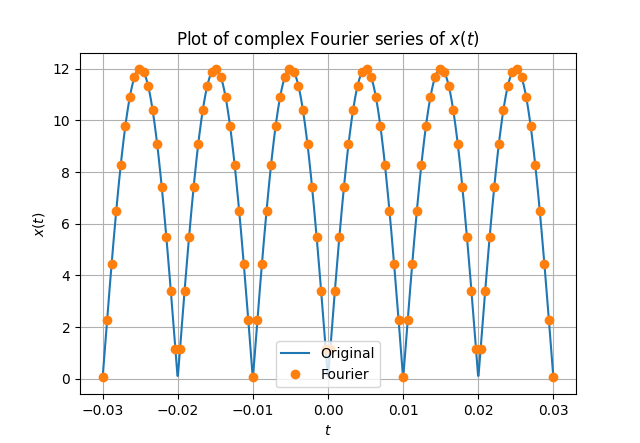
\includegraphics[width=\columnwidth]{./figs/2.3.png}
		\caption{Plot of $x(t)$ along with its complex Fourier series expansion}
		\label{fig-2.3}	
	\end{figure}
	
	\item Show that 
	\begin{align}
		x(t) = \sum_{k = 0}^{\infty}\brak{a_k\cos{\brak{2\pi kf_0 t}}+b_k\sin{\brak{2\pi kf_0 t}}}
		\label{eq:one-Z-real}
	\end{align}
	and obtain the formulae for $a_k$ and $b_k$	
	
	\solution
	\begin{align}
    		x(t) &= \sum_{k = -\infty}^{\infty}c_ke^{\j2\pi kf_0 t} \\
        &= c_0 + \sum_{k = 1}^{\infty}c_ke^{\j2\pi kf_0t} + c_{-k}e^{-\j2\pi kf_0t} 
	\end{align}
	
	Thus
	\begin{multline}
		x(t) = c_0 + \sum_{k = 1}^{\infty}\brak{c_k + c_{-k}}\cos\brak{2\pi kf_0t}   \\
        + \sum_{k = 1}^{\infty}\j\brak{c_k - c_{-k}}\sin\brak{2\pi kf_0t}
	\end{multline}
	
	Therefore
	\begin{align}
    		a_k &= 
	    \begin{cases}
	        c_0 & k = 0 \\
    		    c_k + c_{-k} & k > 0
	    \end{cases} \\
    		b_k &= \j(c_k - c_{-k}) ~~ k \ge 0
	\end{align}	
	
	\item Find $a_k$ and $b_k$ for \eqref{eq:10-orig-diff-def}
	
	\solution 
	\begin{align}
		a_0 &= c_0 = \frac{2A_0}{\pi} 
	\end{align}
	
	For $k > 0$, if $k$ is odd
	\begin{align}
		a_k = 0 + 0 = 0
	\end{align}
	
	and if $k$ is even
	\begin{align}
		a_k = \frac{2A_0}{\pi(1-k^2)} + \frac{2A_0}{\pi(1-k^2)} = \frac{4A_0}{\pi(1-k^2)}
	\end{align}
	
	For odd or even $k$, $c_k = c_{-k}$ always
	\begin{align}
		b_k = 0 \quad \forall k \ge 0
	\end{align}
	
	Therefore
	\begin{align}
		a_k &=
		\begin{cases}
			\frac{2A_0}{\pi} & k = 0 \\
			\frac{4A_0}{\pi(1-k^2)} & k = 2m, m \in \mathbb{N} \\
			0 & \text{otherwise}
		\end{cases} \\
		b_k &= 0 \qquad \quad ~ k \ge 0
	\end{align}
	
	\item Verify \eqref{eq:one-Z-real} using Python
	
	\solution Download the following Python code that plots Fig. \ref{fig-2.6}.
	\begin{lstlisting}
		wget https://github.com/Ankit-Saha-2003/EE3900/raw/main/Fourier/codes/2.6.py
	\end{lstlisting}
	
	Run the code by executing
	\begin{lstlisting}
		python 2.6.py
	\end{lstlisting}

	\begin{figure}[!ht]
		\centering
		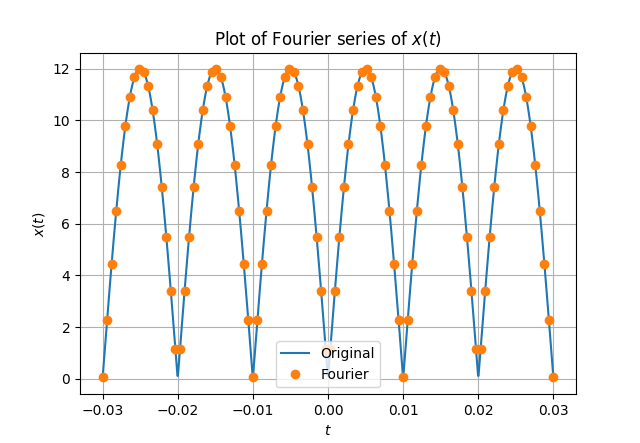
\includegraphics[width=\columnwidth]{./figs/2.6.png}
		\caption{Plot of $x(t)$ along with its Fourier series expansion}
		\label{fig-2.6}	
	\end{figure}
	
	\begin{figure}[!ht]
		\centering
		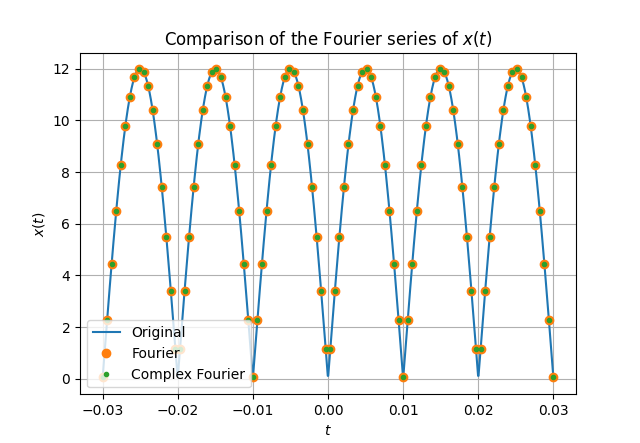
\includegraphics[width=\columnwidth]{./figs/comparison.png}
		\caption{Comparison of the Fourier series of $x(t)$}
		\label{fig-comparison}	
	\end{figure}
	\end{enumerate}

	\section{Fourier Transform}
	\begin{enumerate}[label=\thesection.\arabic*,ref=\thesection.\theenumi]
	\item 
	\begin{align}
		\delta(t) &= 0 && t \ne 0 \\
		\int_{-\infty}^{\infty} \delta(t) \der{t} &= 1
	\end{align}
	
	 \item The Fourier Transform of $g(t)$ is
 	\begin{align}
 		G(f)=\int_{-\infty}^{\infty}g(t)e^{-j2\pi ft}\,\der{t}
 	\end{align}
 	
	\item Show that 
	\begin{align}
		g(t-t_0)&\system{F}G(f)e^{-j2\pi ft_0}
	\end{align}
	\solution 
	\begin{align}
		g(t-t_0) \system{F} &\int_{-\infty}^{\infty}g(t-t_0)e^{-j2\pi ft}\,\der{t} \\
		=& \int_{-\infty}^{\infty}g(u)e^{-j2\pi f(u+t_0)}\,\der{u} \\
		=& e^{-j2\pi ft_0} \int_{-\infty}^{\infty}g(u)e^{-j2\pi fu}\,\der{u} \\
		=& G(f)e^{-j2\pi ft_0}
	\end{align}
	
	\item Show that 
	\begin{align}
		G(t)&\system{F}g(-f)
	\end{align}
	\solution
	\begin{align}
		G(t)&\system{F} \int_{-\infty}^{\infty}G(t)e^{-j2\pi ft}\,\der{t} 
	\end{align}
	But
	\begin{align}
		g(t)&=\int_{-\infty}^{\infty}G(f)e^{\j2\pi ft}\,\der{f} \\
		&= \int_{-\infty}^{\infty}G(u)e^{\j2\pi ut}\,\der{u} \\
		\implies g(-f) &= \int_{-\infty}^{\infty}G(u)e^{-\j2\pi uf}\,\der{u} \\
		&= \mathcal{F}\cbrak{G(t)}
	\end{align}
	
	\item Find the Fourier transform of $\delta(t)$
	
	\solution 
	\begin{align}
		\delta(t)\system{F} &\int_{-\infty}^{\infty}\delta(t)e^{-j2\pi ft}\,\der{t} \\
		=& \left. e^{-j2\pi ft} \right|_{t=0} \\
		=& 1
	\end{align}
	
	\item Find the Fourier transform of $e^{-\j2\pi f_0 t}$
	
	\solution 
	\begin{align}
		\delta(t) &\system{F} 1 \\
		\implies \delta(t-f_0) &\system{F} e^{-j2\pi ff_0} \\
		\implies e^{-j2\pi tf_0} &\system{F} \delta(-f-f_0) \\
		\therefore e^{-j2\pi tf_0} &\system{F} \delta(f+f_0)
	\end{align}
	
	\item Find the Fourier transform of $\cos\brak{2\pi f_0 t}$
	
	\solution 
	\begin{align}
		&\cos\brak{2\pi f_0 t} = \frac{e^{\j2\pi f_0 t} + e^{-\j2\pi f_0 t}}{2} \\
		\implies &\cos\brak{2\pi f_0 t} \system{F} \frac{\delta(f-f_0) + \delta(f+f_0)}{2}
	\end{align}

	\item Find the Fourier transform of $x(t)$ and plot it. Verify using Python

	\solution 
	\begin{align}
		x(t) &= \sum_{k=-\infty}^\infty c_k e^{\j 2\pi kf_0t} \\
		\mathcal{F}\cbrak{x(t)} &= \sum_{k=-\infty}^\infty c_k \mathcal{F}\cbrak{e^{\j 2\pi kf_0t}} \\
		&= \sum_{k=-\infty}^\infty c_k \delta(f-kf_0) \\
		&= \frac{2A_0}{\pi} \sum_{k \text{ is even}} \frac{\delta(f-kf_0)}{1-k^2}
	\end{align}
	
	Download the following Python code that plots Fig. \ref{fig-3.8}.
	\begin{lstlisting}
		wget https://github.com/Ankit-Saha-2003/EE3900/raw/main/Fourier/codes/3.8.py
	\end{lstlisting}
	
	Run the code by executing
	\begin{lstlisting}
		python 3.8.py
	\end{lstlisting}

	\begin{figure}[!ht]
		\centering
		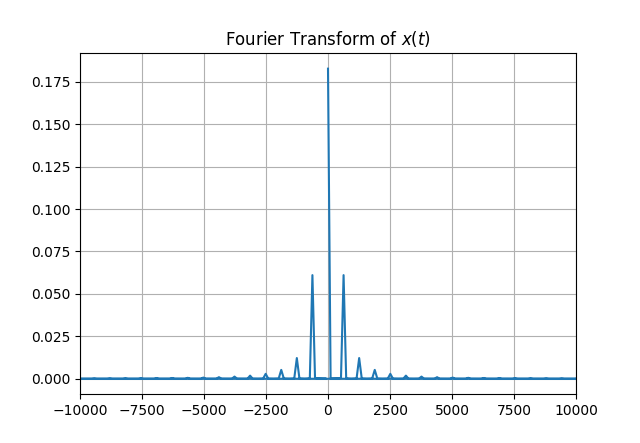
\includegraphics[width=\columnwidth]{./figs/3.8.png}
		\caption{Plot of the Fourier transform of $x(t)$}
		\label{fig-2.3}	
	\end{figure}
	
	 \item Show that 
	 \begin{align}
		 \rect{t} \system{F} \sinc{f}
 	\end{align}
 	Verify using Python
 	
 	\solution
 	\begin{align}
 		\rect{t} = 
 		\begin{cases}
 			1 & \abs{t} \le \frac{1}{2} \\
 			0 & \text{otherwise}
 		\end{cases}
 	\end{align}
 	Its Fourier transform is given by
 	\begin{align}
 		\rect{t} \system{F} &\int_{-\infty}^{\infty}\rect{t}e^{-j2\pi ft}\,\der{t} \\
 		&= \int_{-\frac{1}{2}}^{\frac{1}{2}} e^{-j2 \pi ft} \der{t} \\
 		&= \frac{e^{-j \pi f} - e^{j \pi f}  }{-\j2 \pi f} \\
 		&= \frac{\sin\pi f}{\pi f} \\
 		&= \sinc{f}
 	\end{align}
 	
 	Download the following Python code that plots Fig. \ref{fig-3.9}.
	\begin{lstlisting}
		wget https://github.com/Ankit-Saha-2003/EE3900/raw/main/Fourier/codes/3.9.py
	\end{lstlisting}
	
	Run the code by executing
	\begin{lstlisting}
		python 3.9.py
	\end{lstlisting}

	\begin{figure}[!ht]
		\centering
		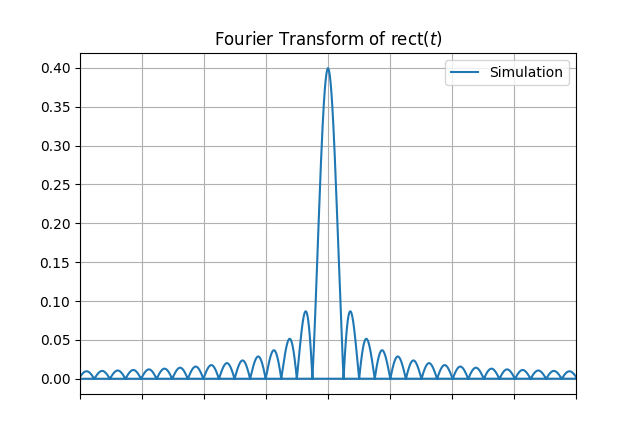
\includegraphics[width=\columnwidth]{./figs/3.9.png}
		\caption{Plot of the Fourier transform of $\rect{t}$}
		\label{fig-3.9}	
	\end{figure}
	
	\item Find the Fourier transform of $\sinc{t}$. Verify using Python
	
	\solution 
	\begin{align}
		\rect{t} \system{F} &\sinc{f} \\
		\implies \sinc{t} \system{F} &\rect{-f} \\
		&= \rect{f}
	\end{align}
	
	Download the following Python code that plots Fig. \ref{fig-3.10}.
	\begin{lstlisting}
		wget https://github.com/Ankit-Saha-2003/EE3900/raw/main/Fourier/codes/3.10.py
	\end{lstlisting}
	
	Run the code by executing
	\begin{lstlisting}
		python 3.10.py
	\end{lstlisting}

	\begin{figure}[!ht]
		\centering
		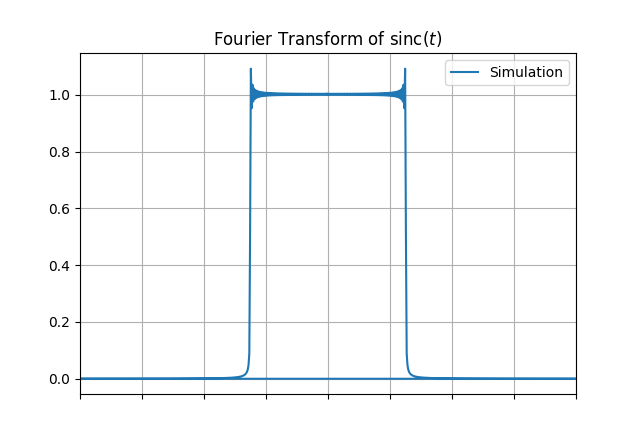
\includegraphics[width=\columnwidth]{./figs/3.10.png}
		\caption{Plot of the Fourier transform of $\sinc{t}$}
		\label{fig-3.10}	
	\end{figure}
	\end{enumerate}
	
	\section{Filter}
	\begin{enumerate}[label=\thesection.\arabic*,ref=\thesection.\theenumi]
	\item Find $H(f)$ which transforms $x(t)$ to DC \SI{5}{\volt}
	
	\solution Since we want a DC output, the filter we need is a low-pass filter that only lets the zero frequency component pass through, i.e., the amplitude of a  frequency components with a frequency higher than the cutoff frequency $f_c$ has to be zero
	
	We can use a rectangular filter for this purpose
	\begin{align}
		H(f) = k\,\rect{\frac{f}{2f_c}} =
		\begin{cases}
			k & \abs{f} \le f_c \\
			0 & \text{otherwise}
		\end{cases}
	\end{align}
	
	Now
	\begin{align}
		H(0) = \frac{Y(0)}{X(0)}
	\end{align}
	where $Y(k)$ and $X(k)$ are the Fourier transforms of the output \SI{5}{\volt} DC and the input signal respectively
	\begin{align}
		k &= \frac{5}{\frac{2A_0}{\pi}} = \frac{5\pi}{2A_0} \\
		\therefore H(f) &= \frac{5\pi}{2A_0}\rect{\frac{f}{2f_c}}
	\end{align}
	
	
	\item Find $h(t)$
	
	\solution 
	\begin{gather}
		\sinc{t} \system{F} \rect{f} \\
		\implies \sinc{2f_ct} \system{F} \frac{1}{2f_c}\rect{\frac{f}{2f_c}} \\
		\implies \frac{5\pi}{2A_0} 2f_c \sinc{2f_ct} \system{F} \frac{5\pi}{2A_0}\rect{\frac{f}{2f_c}} \\
		\therefore h(t) = \frac{5\pi f_c}{A_0} \sinc{2f_ct}
	\end{gather}
	
	\item Verify your result using  through convolution
	
	\solution Download the following Python code that plots Fig. \ref{fig-4.3}.
	\begin{lstlisting}
		wget https://github.com/Ankit-Saha-2003/EE3900/raw/main/Fourier/codes/4.3.py
	\end{lstlisting}
	
	Run the code by executing
	\begin{lstlisting}
		python 4.3.py
	\end{lstlisting}

	\begin{figure}[!ht]
		\centering
		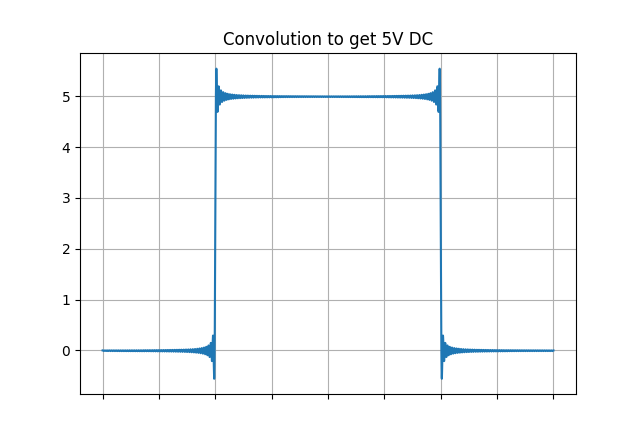
\includegraphics[width=\columnwidth]{./figs/4.3.png}
		\caption{Plot of the convolution of $x(t)$ and $h(t)$}
		\label{fig-4.3}	
	\end{figure}
	\end{enumerate}
	
	\section{Filter Design}
	\begin{enumerate}[label=\thesection.\arabic*,ref=\thesection.\theenumi]
	\item Design a Butterworth filter for $H(f)$
	
	\solution The transfer function of a Butterworth filter is given by
	\begin{align}
		\abs{H_n(f)} = \frac{1}{\sqrt{1+\brak{\frac{f}{f_c}}^{2n}}}
	\end{align}
	where $n$ is the order of the filter and $f_c$ is the cutoff frequency
	
	Let the passband and stopband frequency thresholds be $\SI{50}{\hertz}$ and $\SI{100}{\hertz}$ and their corresponding attenuations be $-\SI{1}{\decibel}$ and $-\SI{5}{\decibel}$ respectively
	\begin{align}
		A_p &= 10 \log_{10}\abs{H_n(f_p)}^2 \\
		&= -10\log_{10}\brak{1+\brak{\frac{f_p}{f_c}}^{2n}} \\
		A_s &= -10\log_{10}\brak{1+\brak{\frac{f_s}{f_c}}^{2n}} \\
		\implies n &=\frac{\log\brak{\frac{10^{-\frac{A_p}{10}}-1}{ 10^{-\frac{A_s}{10}}-1}}}{2 \log \brak{\frac{f_p}{f_s}}} \approx 1.53
	\end{align}
	
	Hence, we choose a $2^{\mathrm{nd}}$ order Butterworth filter with
	\begin{align}
		f_c = \frac{f_p}{\brak{10^{-\frac{A_p}{10}}-1}^{\frac{1}{2n}}} \approx \SI{77.74}{\hertz}
	\end{align}

	\item Design a Chebyschev filter for $H(f)$	
	
	\solution The transfer function of a Chebyshev filter is given by
	\begin{align}
		\abs{H_n(f)} =\frac{1}{\sqrt{1+\epsilon^{2}T_{n}^2\brak{\frac{f}{f_c}}}}
	\end{align}
	where $\epsilon$ is the ripple factor, $f_c$ is the cutoff frequency and $T_n$ is a Chebyshev polynomial of the $n^{\mathrm{th}}$ order
	
	Assuming the same parameters as before along with a ripple of $\SI{0.1}{\decibel}$, we get
	\begin{align}
		\epsilon = \sqrt{10^{\frac{\delta}{10}} - 1} \approx 0.15
	\end{align}
	
	Also, assume that $f_c = f_p \implies \frac{f_s}{f_c} > 1$
	\begin{align}
		&A_s = -10\log_{10}\brak{1+\epsilon^{2}T_{n}^2\brak{\frac{f_s}{f_c}}} \\
		\implies &T_{n}\brak{\frac{f_s}{f_c}} = \frac{\sqrt{10^{-\frac{A_s}{10}} - 1}}{\epsilon} \\
		\implies &\cosh\brak{n\cosh^{-1}\brak{\frac{f_s}{f_c}}} = \frac{\sqrt{10^{-\frac{A_s}{10}} - 1}}{\epsilon} 
	\end{align}
	
	Thus
	\begin{align}
		n = \frac{\cosh^{-1}\brak{\frac{\sqrt{10^{-\frac{A_s}{10}} - 1}}{\epsilon} }}{\cosh^{-1}\brak{\frac{f_s}{f_c}}} \approx 2.26
	\end{align}
	
	Hence, we choose a $3^{\mathrm{rd}}$ order Chebyshev filter
	
	\item Design a circuit for your Butterworth filter
	
	\solution Using the table of normalized Butterworth coefficients, we can see that for a $2^{\mathrm{nd}}$ order Butterworth filter
	\begin{align}
		C_1 &= \SI{1.4142}{\farad} \\
		L_2 &= \SI{1.4142}{\henry}
	\end{align}
	
	On denormalizing these values, we get
	\begin{align}
		C_1' &= \frac{C_1}{2\pi f_c} = \SI{2.89}{\milli\farad} \\
		L_2' &= \frac{L_2}{2\pi f_c} = \SI{2.89}{\milli\henry}
	\end{align}
	
	\begin{figure}[!ht]
    \centering
    \begin{circuitikz} 
        \draw (0,0) to[short, o-o] (4,0);
        \draw (1,0) to[C, l=\SI{2.89}{\milli\farad}] (1,2);
        \draw (0,2) to [short, o-] (1,2) 
        		to [L, l=\SI{2.89}{\milli\henry}] (3.5,2) 
        		-- (4,2) to[short, -o] (4,2);      
    \end{circuitikz}
    \caption{$2^{\mathrm{nd}}$ order Butterworth filter circuit}
    \label{ckt:butter}
	\end{figure}
	
	\item Design a circuit for your Chebyschev filter
	
	\solution Using the table of normalized Chebyshev coefficients, we can see that for a $3^{\mathrm{rd}}$ order Chebyshev filter
	\begin{align}
		C_1 &= \SI{1.4328}{\farad} \\
		L_2 &= \SI{1.5937}{\henry} \\
		C_3 &= \SI{1.4328}{\farad}
	\end{align}
	
	On denormalizing these values, we get
	\begin{align}
		C_1' &= \frac{C_1}{2\pi f_c} = \SI{4.56}{\milli\farad} \\
		L_2' &= \frac{L_2}{2\pi f_c} = \SI{5.07}{\milli\henry} \\
		C_3' &= \frac{C_3}{2\pi f_c} = \SI{4.56}{\milli\farad}
	\end{align}
	
	\begin{figure}[!ht]
    \centering
    \begin{circuitikz} 
        \draw (0,0) to[short, o-o] (5,0);
        \draw (0,2) to [short, o-] (1,2) 
        		to [L, l=\SI{5.07}{\milli\henry}] (3.5,2) 
        		-- (5,2) to[short, -o] (5,2);
        \draw (1,0) to[C, l=\SI{4.56}{\milli\farad}] (1,2);
        \draw (3.5,0) to[C, l=\SI{4.56}{\milli\farad}] (3.5,2);
    \end{circuitikz}
    \caption{$3^{\mathrm{rd}}$ order Chebyshev filter circuit}
    \label{ckt:cheby}
	\end{figure}
	
	\end{enumerate}
	\end{document}